\documentclass{article}
\usepackage{amsmath}
\usepackage{amsfonts}
\usepackage{graphicx}
\usepackage[utf8]{inputenc}
\usepackage{parskip}

\setcounter{secnumdepth}{2}

\author{Jack Morgan}
\title{Visualisation of the Riemann Hypothesis}

\begin{document}

\maketitle
\clearpage
\section{Analysis}

\subsection{Introduction}

\subsubsection{Project Proposal}

Throughout this coursework, I will be examining the Riemann Hypothesis; to be able to visualise this important conjecture and make its complex mathematical structures accessible for anyone who is interested in mathematics. This project will be heavily based on how to compute and plot recursive mathematical functions on the complex plane and test whether the Riemann hypothesis is a true statement, as well as how the hypothesis affects mathematics today.

\subsubsection{Abstract}

During this coursework, I aim to be able to make the Riemann Hypothesis a more accessible mathematical concept to be able to help people to understand it and hopefully inspire them to research further into related mathematical subjects. I will do this in 3 simple ways:
\begin{enumerate}
\item By detailing what the Riemann hypothesis is and why it is so important,
\item Investigating the major functions that make up the Riemann Hypothesis
\item By Visualising the significant concepts of the Hypothesis, in order to make them more understandable; and to be able to investigate what they are and how they work.
\end{enumerate}

I will be conducting my investigation by programming the key functions of the Hypothesis in Python 3. This will allow me to:
\begin{enumerate}
\item Compute key mathematical functions
\item Plot graphs of data
\item Store data in files and a database
\item Have a guided user interface
\end{enumerate}

\subsubsection{End Users}

This project is aimed at people who are interested in mathematics. It is a great way to inspire people to delve deeper into maths and number theory; as well as help those with a more advanced understanding of mathematics. Although the mathematics and understanding behind the problem can be complex at times, I am for this project to be able to be used by anyone who will want to use it. This would require it to be simple for people to understand and navigate. I aim to get input from people with a range of mathematical abilities to give me feedback on the project.


\subsection{Research}

\subsubsection{What is the Riemann Hypothesis?}

The Riemann Hypothesis - first proposed by Bernhard Riemann in 1859 - is considered by many to be one the most important unsolved problems in mathematics. To understand why the Riemann hypothesis is so important, it is necessary to understand what the Riemann hypothesis is, and how it is used in many mathematical and scientific fields.
The Riemann hypothesis was proposed by Bernhard Riemann in his paper "On the Number of Primes Less Than a Given Magnitude". This paper deeply explores the prime numbers, and the functions used to estimate and count prime numbers. Throughout this paper, Riemann discussed definitions and proofs of multiple theories that all relate to the prime numbers. But most notably, he had taken a function previously mentioned by Leonhard Euler (a famous mathematician who lived around 100 years prior), and formalised this function into the Riemann Zeta Function.


Riemann took Euler’s function and used a process called analytic continuation to extend the domain of this function to all numbers - be that real, imaginary or complex. Just like every other function, the Riemann Zeta Function contains what are called ‘zeros’ or ‘roots’. This is where a function’s output is equal to zero. These zeros can be described as trivial (where the explanation for why these zeros exist is almost intuitive), or non-trivial (where it can be hard to explain why these zeros occur.) The Riemann Zeta Function has trivial zeros when the input is a negative even integer. I will explore why this is the case later on. However, the non-trivial zeros of the zeta function can be found when the real part of the function’s input is between 0 and 1 (called the critical region). This is a fact that has been proven by Riemann in his paper, and he even proved that there are an infinite amount of non-trivial zeros in the critical region. But Riemann went further than this, he hypothesised that the non-trivial zeros do not only occur when the real part of the input is between 0 and 1; but they all occur in the middle of the critical region when the real part of the input is exactly ½. The Riemann Hypothesis states that ‘the real part of every nontrivial zero of the Riemann zeta function is ½’. This is the fundamental part of the Riemann Hypothesis, and although it is widely considered to be true, this conjecture has never actually been proven with conclusive evidence, and that is why these are considered to be non-trivial zeros.
\begin{figure}
\centering
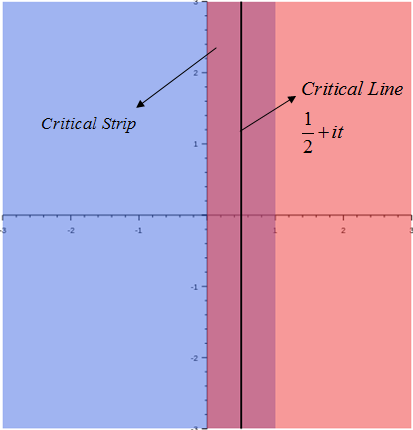
\includegraphics[scale=0.4]{critical-strip}
\caption{Critical Strip and Line}
\end{figure}
\subsubsection{The Importance of the Riemann Hypothesis}
The Riemann Hypothesis and the  Riemann Zeta Function have many extraordinary uses. From calculating prime numbers to uses in Quantum Physics, and even cryptography with the RSA algorithm. This is due to the fact that the Zeta function is deeply connected to the prime numbers.

One of the main reasons why the Riemann Hypothesis is significant is because there have been many conjectures and theories that assume the Riemann hypothesis to be true. So if the Riemann hypothesis was proven, this would also prove countless other theories.
Some of these theories include :
\begin{itemize}
\item The weak Goldbach conjecture - stating that all integers greater than 5 are the sum of three primes
\item Mills’ constants - numbers that allow you to generate prime numbers
\item The theory that there will always be at least one prime between consecutive cubes
\item The theory that there is a maximum bound between consecutive prime numbers
\end{itemize}
All of these theories are, in some way, related to the prime numbers. There is an important reason for this which I’ll cover in a later section.

If the Riemann Hypothesis was proven to be true, there would be profound effects in fields such as cryptography. In public-key cryptosystems, like RSA, public keys are created using prime numbers. If someone wanted to try and decode information without knowing what the prime numbers were that created the key, they would have to try and guess what the prime numbers were. What keeps these algorithms secure is the fact that it can take a long time to calculate the prime numbers, especially some of the larger ones. In fact, the largest prime number discovered has over 23 million digits. However, if the Riemann hypothesis were true, then people would be able to calculate the prime numbers much quicker than before. This would make many of the current cryptography algorithms obsolete.

The Riemann Hypothesis does not just influence mathematics and cryptography, it also has great importance in quantum physics. It was discovered in 1996 that the arrangement of the zeta zeros exhibits the same statistical pattern as the spectra of energy levels (that is the possible values of energy of a quantum system) in quantum chaotic systems. Furthermore, it was conjectured in 1999 by Michael Berry and Jonathan Keating, that there will exist a quantum system, where the energy levels will correspond exactly to the non-trivial zeros of the Riemann Zeta Function. If this conjecture is true, it would prove the Riemann Hypothesis.

\subsubsection{Complex Numbers and Key Operations}
Complex numbers play a key part in the Riemann Hypothesis. When Riemann created the Riemann Zeta Function, he allowed the inputs and outputs to be complex numbers, through his ideas of analytic continuation. It is therefore important to know what complex numbers are, and how to do arithmetic with them.

To first understand complex numbers (denoted by the symbol $\mathbb{C}$), it is necessary to be familiar with the idea of imaginary numbers. There is no real number whose square root is a negative number, so mathematicians decided to invent numbers for this. It is denoted by the symbol i, for the imaginary unit.

Where: $$i \equiv \sqrt{-1}$$
And thus: $$i^2 \equiv -1$$
You can multiply the imaginary unit($i$) by any real number to create an imaginary number. For example:
$$3i$$
$$2i$$
Which are both imaginary numbers.
By combining both real numbers and imaginary numbers, you can create complex numbers.
For example:
$$2+3i$$
Where the real part of the number is $2$, and the imaginary part is $3i$.
$$4-7i$$
Where the real part of the number is $4$, and the imaginary part is $-7i$.
We often represent real numbers on a number line, however, this is impossible to do with complex numbers. Instead, one way to understand them is through a two-dimensional graph, or to give it its formal name, the complex plane. On the complex plane, there are two axes, a real axis and an imaginary axis. Any complex number can be plotted on the complex plane. We can think of a complex number as a set of coordinates that tell us where the number lies on the complex plane, with the real part being the x coordinate and the imaginary part being the y coordinate.

So if we wanted to plot the point $2+3i$ on the complex plane, it would look as follows:

\begin{figure}
\centering
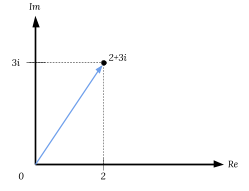
\includegraphics[scale=1]{argand diagram 23i}
\caption{Critical Strip and Line}
\end{figure}

This type of diagram is known as an Argand Diagram. And as you can see, we have plotted the point $2+3i$ at the coordinates $(2, 3)$ on the complex plane.

We can also do arithmetic with complex numbers - be that addition, subtraction, multiplication, division or exponentiation.

The sum of two complex numbers is the sum of both of the real parts of the numbers, plus the sum of the two complex parts of the numbers.
$$(3+2i) + (1+3i)$$
$$= (3+1) + (2i+3i)$$
$$= 4 + 5i$$

Subtraction is also done using a similar method.

$$(3+2i)-(1+3i)$$
$$=(3+2i) + (-1-3i)$$
$$=(3-1)+(2i-3i)$$
$$=2-i$$

To multiply two complex numbers, it is equivalent to expanding out two binomial brackets where:

$$(a+b)(c+d)$$
$$= ac + ad + bc + bd$$

So with two complex numbers this would look like:

$$(3+i)(2+2i)$$
$$= 6 + 6i + 2i + 2i^2$$
$$= 6 + 8i + 2i^2$$

We can then use the identity $i^2 \equiv -1$ to simplify this expression, so that:

$$= 6+8i + 2(-1)$$
$$= 4 + 8i$$

But we can speed up this method by using the rule $(a+bi)(c+di) = (ac-bd)+(ad + bc)i$
For example:
$$(3+i)(2+2i)$$
$$= (32 - 12) + (32 + 12)i$$
$$= 4+8i$$
We can derive this rule, to prove that it works for all complex numbers:
\begin{align*}
RTP: (a+bi)(c+di) &= (ac-bd)+(ad+bc)i\\
LHS &=  (a+bi)(c+di)
\intertext{Distributing Terms:}\\
&=ac + adi + bci + bdi^2\\
\intertext{Using $i^2=-1$:}\\
&=ac + adi + bci -bd\\
\intertext{Then rearranging:}\\
&= ac-bd + adi + bci\\
&= (ac-bd)+(ad+bc)i\\
&= RHS\\
&\text{    }Q.E.D
\end{align*}

% \subsection{Project Objectives}

% \subsection{Third-Party Input}

% \subsection{Modelling the Problem}

% \section{Documented Design}

\end{document}
